\documentclass[journal]{./IEEE/IEEEtran}
\usepackage{cite,graphicx, caption, url}


\newcommand{\SPTITLE}{SkyLab : A Web Application for vCluster}
\newcommand{\ADVISEE}{Vincent Paul L. Carpio}
\newcommand{\ADVISER}{Katrina Joy M. Abriol-Santos}
\newcommand{\ADVISERR}{Joseph Anthony C. Hermocilla}

\newcommand{\BSCS}{Bachelor of Science in Computer Science}
\newcommand{\ICS}{Institute of Computer Science}
\newcommand{\UPLB}{University of the Philippines Los Ba\~{n}os}
\newcommand{\REMARK}{\thanks{Presented to the Faculty of the \ICS, \UPLB\
                             in partial fulfillment of the requirements
                             for the Degree of \BSCS}}

\markboth{CMSC 190 Special Problem, \ICS}{}
\title{\SPTITLE}
\author{\ADVISEE~and~\ADVISER~and~\ADVISERR%
\REMARK
}
\pubid{\copyright~2016~ICS \UPLB}

%%%%%%%%%%%%%%%%%%%%%%%%%%%%%%%%%%%%%%%%%%%%%%%%%%%%%%%%%%%%%%%%%%%%%%%%%%

\begin{document}

% TITLE
\maketitle

\begin{abstract}
	Most scientific applications require high performance computing (HPC) which utilizes parallel processing to run tasks quickly and efficiently. MPI clusters are often used to cater this type of tasks but the hardware required can be costly. Peak-Two Cloud (P2C) can host HPC applications in a cloud environment which is relatively cheaper and more convenient. One of its features is vCluster, a tool that can deploy MPI clusters on demand. \cite{Hermocilla2014} We have developed SkyLab, a web interface for vCluster. It aims to simplify the process of running MPI tasks from the perspective of the end-user. Here, we describe the system design and features of SkyLab. 
\end{abstract}
% ABSTRACT

% INDEX TERMS
\begin{keywords}
cloud computing, high performance computing, web interface
%key, words, separated, by, comma
\end{keywords}

% INTRODUCTION
\section{Introduction}
	\subsection{Background}
	Cloud computing has marked significant developments and possibilities in the industry. It focuses on offering services for the different needs of the modern society.
	% detected
	 There are three categories of cloud computing services namely, Software as a Service (SaaS), Platform as a Service (PaaS) and Infrastructure as a Service (IaaS). Organizations provide Saas depending on the demand. Google Apps is one example of Saas that can be used to manage email and create documents, etc. Paas offers developers a platform where they can build and deploy applications. Iaas provides storage, servers and handling computer clusters. These tools are primarily created to serve computational needs \cite {Ahuja2012}. A cloud computing platform dynamically allocates, configures, reconfigures and deallocates servers as requested or on demand. This approach ensures the elasticity of cloud computing \cite {Brandic2011}.

	Most scientific applications require high performance computing (HPC) which needs CPU intensive computations and large data storage. To be able to host such applications, several computers interconnected in a network such as clusters are needed. This makes scientific computing very costly. Fortunately, with the advancement in cloud computing, these tools can be deployed in the cloud without worrying about the costs of hardware purchase and maintenance \cite {Ahuja2012}. To determine the cost of hosting scientific computing in cloud, the Scientific Computing Cloud (SciCloud) project is conducted in the University of Tartu. Results have shown that transmission delays are the major concern in pursuing HPC applications in the cloud\cite {Brandic2011}.  To address this problem, a study is conducted by Hermocilla in Peak-Two Cloud (P2C). One of the features introduced by P2C is vCluster. vCluster is a tool that enables a user to deploy a working MPI cluster on demand and to terminate it after execution. It uses a master-slave design implementation \cite {Hermocilla2014}. However, vCluster is a command-line based application which has limited capacities for data manipulation, analysis, and presentation. Creating a web application that would host vCluster with additional features like graphical representation to visualize trends, and a Graphical User Interface(GUI) to offer convenient access. This paper will present SkyLab, a web application that aims to serve and to improve vCluster functionalities.

    \subsection{Significance of the Study}
    This study will help us visualize how HPC applications can be hosted in the cloud and understand why is this technology timely relevant.  Even with capable hardware, computations might take hours or even days which makes it a hassle for users. Thus, there is a need for a more convenient way of access for HPC applications. Furthermore, this would encourage students to explore and research on HPC applications. HPC applications usually have a plain numerical output. A means of presenting data graphically would make the interpretation of data more efficient.

    The study would contribute to research on hosting HPC applications in the cloud. Problems encountered and solutions offered throughout the study will give insights to future researchers. Furthermore, the output application of the study can be used by the academe.

    \subsection{Scope and Limitations}
    The study focuses on vCluster and is not mainly concerned on P2C as a whole. The study initially bases on the current implementation of vCluster and eventually improve it and offer additional features\cite {Hermocilla2014}.

    \subsection{Objectives}
    This study aims to develop SkyLab, a web application that would function as a front-end for vCluster. %change support
	Specifically, it should be able to: 
	\begin{enumerate}
	
		\item allow users to select tools and execute them via web interface; 
        \item create an extensible platform that would accommodate additional tools; and
		\item display output data of tools.
	\end{enumerate}

%REVIEW OF RELATED LITERATURE
\section {Review of Related Literature}
    \subsection{Performance Concerns for HPC Applications in the Cloud}
        Shajulin \cite {8521133920130201} has enumerated five performance concerns for HPC applications in the cloud. First concern is resource provisioning issues which includes memory management, \newline \newline energy management, response time, and resource outages.  Hardware virtualization for multiple guest operating systems running concurrently on a host computer creates a concern for huge overheads, delays, or memory leakages caused by the process of allocating memory, remapping it to virtual machines, and cleaning the memory. The scenario of multiple guest OS can also cause an OS to fail to make hardware use energy-efficient due to lack of control over hardware resources. Configuration failures, update failures, or even unknown issues cause resource outages. Second, most programming models used in the cloud have inconsistencies between the fault recovery mechanisms in execution and  storage processes. Inconsistencies can result to poor performance. Third, enforcing terms of Service Level Agreement (SLA) is bound to performance issues due to loss of control over resource provisioning or deploying cloud services. Fourth, lack of best practices or standards has hindered the utilization of the cloud. If there is no standard interoperable cloud interfaces, users might need to modify their application accordingly with the cloud provider. Fifth, security measures challenges performance since increasing security protocols decreases response time \cite {8521133920130201}.

         In a study by Jackson et al.\cite{CloudCom2010}, performance of a set of benchmarks designed to represent a typical HPC workload run on Amazon EC2 have been quantitatively examined. Results of the study show that the percentage of the communication time of the application is strongly correlated to its overall performance in EC2. The more communication, the worse it performs. In addition, applications with significant global communication perform relatively worse than those with less. Lastly, variability can be significant in EC2. Variability is introduced by multiple virtual machines, by the network and by underlying non-virtualized hardware \cite{CloudCom2010}.

         Another study conducted by  \cite{juve_scientific_2009}, analyzed running scientific workflows in EC2. It has been found that the primary cost is in getting resources to execute workflow tasks, and storage costs are relatively cheaper. Storing data in the cloud rather that transferring it to each workflow effectively reduces the high cost of data transfer. These results show that the cloud is a good alternative for running scientific workflow applications but for cloud providers to be able compete with existing physical systems in terms of performance of HPC applications would need high-speed networks and parallel file systems \cite{juve_scientific_2009} \cite{WalkerEC2HPC}. While current cloud computing services are insufficient for large-scale scientific computing, it may still be a viable option for the scientists who need resources instantly and temporarily \cite{PerfAnalysisManyTasks}. Despite the performance trade-off, EC2 offers ease-of-use and cheaper costs which are marginal factors in consideration for academic purposes \cite{ZachHumphrey}.
    \subsection {Related Work}
        The Yabi system \cite{7411021620120101} targets the non-technical audience with an intuitive drag-and-drop scalable web-based workflow environment that allows HPC to be appreciated a broader audience. Yabi also enables other workflow systems that have limited access to multiple existing HPC to utilize its data and access models.
        
	Another related project is WImpiBLAST\cite{9686120720140601}, an open-source web interface for parallel BLAST searches. BLAST is the most extensively used gene sequence analysis program for sequence homology similarity search in large databases of sequences. mpiBLAST is an open-source parallelization of BLAST that can speedup large-scale annotation by using supercomputers and HPC clusters. WImpiBLAST is created to help researchers who lack expertise in using Message Passing Interface (MPI) benefit from its advantages.     
        
        
\section{Methodology}
   \subsection {Materials}
    \begin{description}
      \item[Programming Language: Python ]
      \item[Web Framework: Django ]
      \item[DBMS: MariaDB]
      \item[Cloud Infrastructure: Peak-Two Cloud ]
    \end{description}


    \subsection{System Architecture}
    SkyLab functions as a web front-end for vCluster which is built on top of Peak-Two Cloud.
   	\begin{center}			
		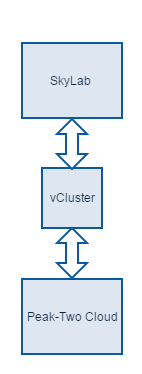
\includegraphics[width=92px,height=224px]{./images/system_architecture.png}			
		\captionof{figure}{System Architecture of SkyLab}			
	\end{center}	
    

   % 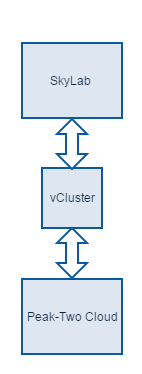
\includegraphics {./images/system_architecture.png}


%	\begin{center}			
%		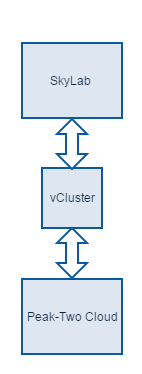
\includegraphics[width=92px,height=224px]{./images/system_architecture.png}			
%		\captionof{figure}{System Architecture of SkyLab}			
%	\end{center}	
	
    \begin{figure*}[ht]
      \centering
      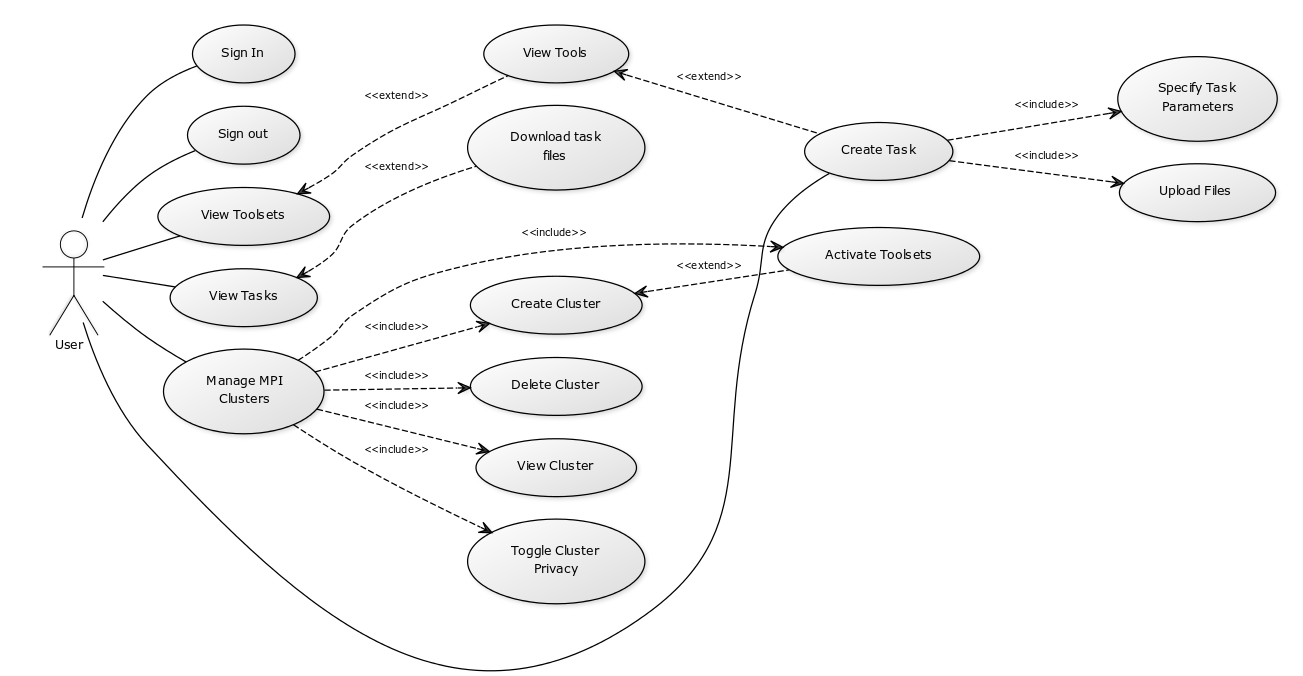
\includegraphics[width=500px,height=250px]{./images/use_case_large.png}
      \caption{Use Case Diagram of SkyLab}\label{System Architecture}
    \end{figure*}

    \subsection{Requirements Specification}
        \subsubsection{Functional Requirements}
        \begin{itemize}
          \item Users can browse and select tools with an interface. It includes, but not limited to:
          \begin{description}
          	\item[AutoDock] \hfill \break 
            It is a suite of automated docking tools designed to predict how small molecules bind to a receptor of known 3D structure. \cite{morris2009autodock4}
            \item[AutoDock Vina] \hfill \break
            It achieves significant improvements in the average accuracy of the binding mode predictions, while also being up to two orders of magnitude faster than AutoDock 4. \cite{JCC:JCC21334}
            \item[DOCK] \hfill \break
            It is used to predict the small molecule-target interactions. \cite{lang2009dock}
            \item[Quantum Espresso] \hfill \break
It is an integrated suite of Open-Source computer codes for electronic-structure calculations and materials modeling at the nanoscale. \cite{QE-2009}
            \item[GAMESS] \hfill \break
            GAMESS is a program for ab initio molecular quantum chemistry. \cite{1993gamess}
            \item[Ray] \hfill \break
            It is uses parallel genome assemblies for parallel DNA sequencing \cite{boisvert_ray_2012}
          \end{description}
          \item Users can upload input data to the server.
          \item Users can view the results of the used tools.
          \item The system is integrated with vCluster functionalities.
        \end{itemize}
        \subsubsection{Non-functional Requirements}
        \begin{itemize}
          \item Users must be authenticated to be able to use the system.
          \item The system must be easy to use and user friendly.
          \item The system must be highly maintainable for future development.  
        \end{itemize}
	
    \subsection {Evaluation of Methodology}
    	The use cases given ensure that the user will be able to select tools and execute them with the system. Also, the output files of user tasks will be served by the system. The system code is required maintainable for future inclusion of other tools.  
        The methodology provided is sufficient to achieve the given objectives of the study. The created software will be subjected to user acceptance test for further evaluation. 

\section{Results and Discussion}
	\subsection{System Design}
		\subsubsection{MPI clusters} 
		The system spawns a thread (MPIThread) for each active cluster which handles the connection to the assigned cluster via Secure Shell (SSH). Creation and deletion of clusters is done by using vCluster commands while tool activation is done by using p2c-tools. The thread also manages task queuing and execution.
		
		A cluster is either classified as public or private. If it is set to public, every user in the system can use it. On the other hand, for private clusters, the cluster will only be visible to the owner. The owner has the option to share the cluster to other users via the share key generated for the said cluster. 		

		\subsubsection{Tool Sets} 
		The system searches for Python packages inside the assigned modules folder and install it on server start. The tool sets will then be available for use with the system. The package must have a Python module named \emph{install.py} which contains function calls for integrating the package with the system. The package must also contain the corresponding views and executable classes for each sub-tool  

		\subsubsection{Tasks} 
		The system creates a task object for each task input by the user. A signal will then be sent and it is then received by the corresponding MPIThread which queues the task for execution. When a task is executed, it calls the assigned executable class with the given parameters. On connection error, the task waits exponentially before retrying. If the server crashes while running task execution, the task is just restarted.				
		
		 Default task execution flow via executable class:			
		\begin{enumerate}
			\item  Needed remote and local directories for execution are cleared or created.
			\item  Input files are uploaded to cluster.
			\item  List of commands given are executed.
			\item  Output files are sent back to the server.
			\item  Deletes remote task folder
			\item  Output files are served by the server.
		\end{enumerate}	

	\subsection{System Features}
	The system's interface offers different functionalities that simplifies MPI cluster and task management.
		
	\begin{itemize}
		\item The user is authenticated by logging in with his @up.edu.ph Google account.
		\item The user can create an MPI cluster with optional tool activations. 
			\begin{center}			
				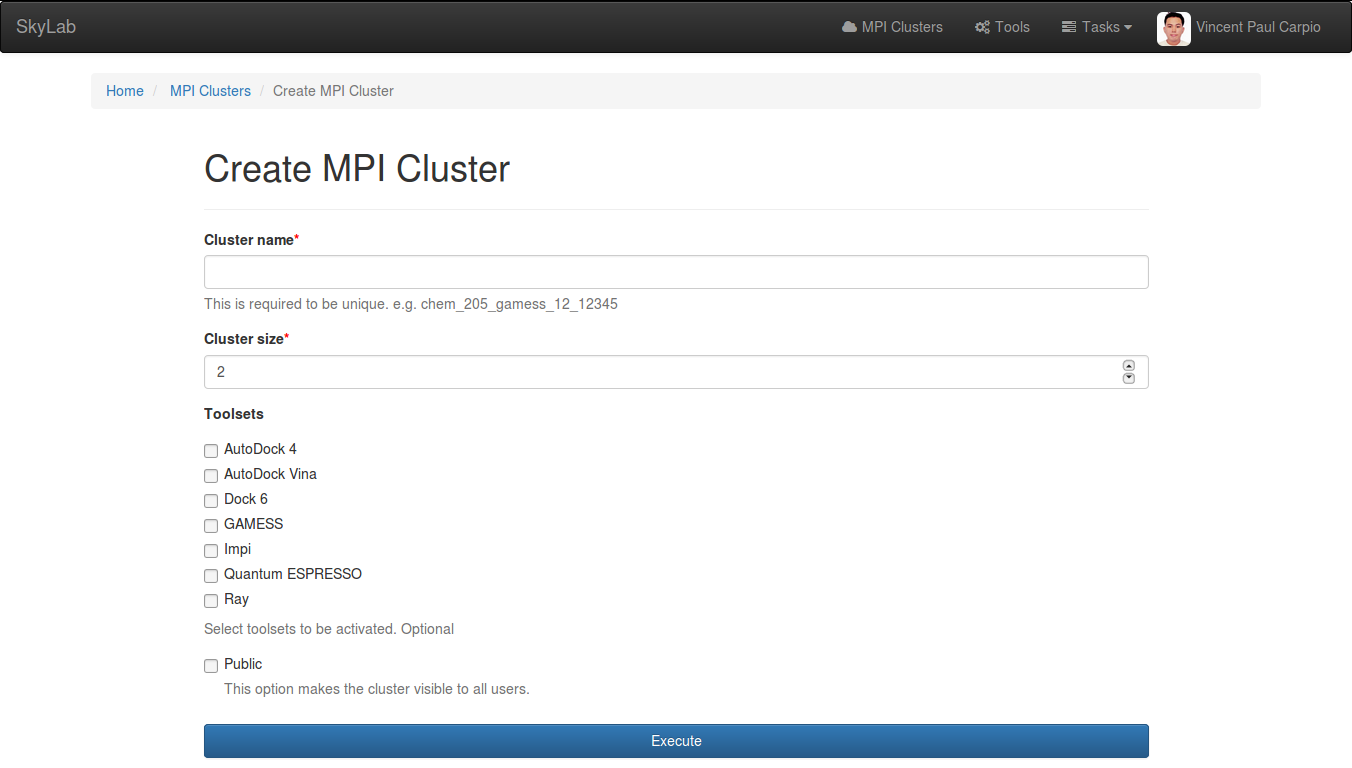
\includegraphics[scale=0.50]{./images/create_mpi.png}				
				\captionof{figure}{MPI creation form}			
			\end{center}	
	
		\item The user can monitor visible public and private MPI clusters.  \newline	
		\begin{center}			
			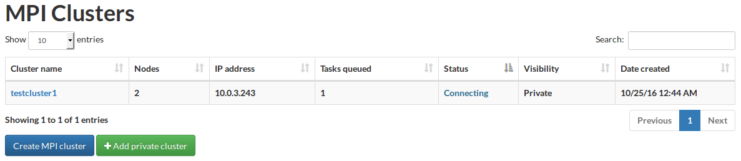
\includegraphics[scale=0.33]{./images/mpi_list_view.png}				
			\captionof{figure}{MPI cluster table}		
		\end{center}
		
	
		\item The user can make a private cluster visible by entering a valid share key. \newline
		\begin{center}			
			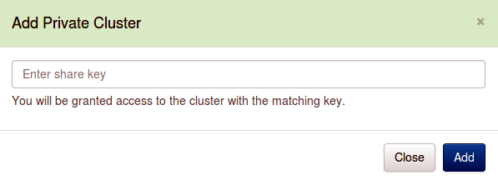
\includegraphics[scale=0.50]{./images/add_private_cluster_2.png}		
			\captionof{figure}{Add private cluster form}			
		\end{center}	
		
		\item The user can view details about a MPI cluster. If the user is the cluster's owner he has the option to delete the cluster. \newline
		\begin{center}			
			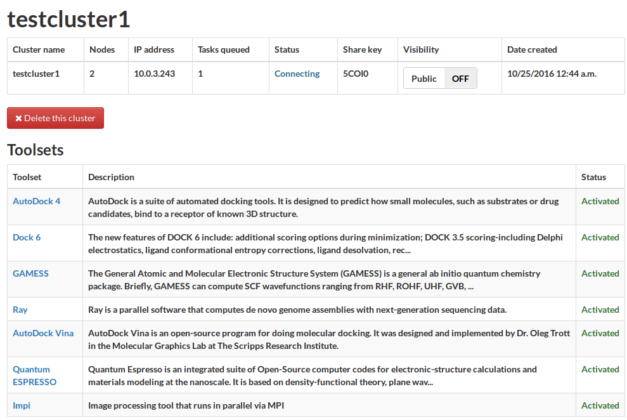
\includegraphics[scale=0.40]{./images/mpi_detail_view_2.png}			
			\captionof{figure}{MPI detail view}			
		\end{center}	
		
		\item The user can select from a list which tool does he want to use. 	
		\begin{center}			
			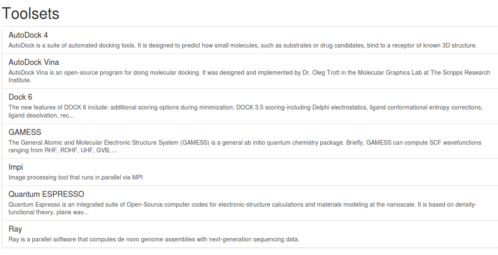
\includegraphics[scale=0.45]{./images/toolset_list_2.png}			
			\captionof{figure}{Tool set list view}			
		\end{center}
		
		\item The user can submit a task by filling up a tool's task creation form. \newline
		\begin{center}			
			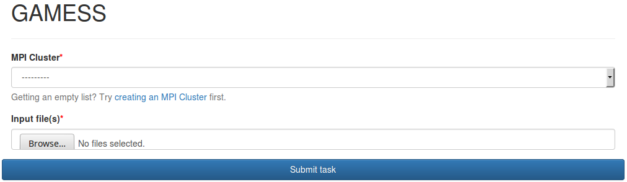
\includegraphics[scale=0.40]{./images/gamess_form_2.png}			
			\captionof{figure}{GAMESS task creation form}			
		\end{center}	
		
		\item The user can monitor created tasks. \newline
		\begin{center}			
			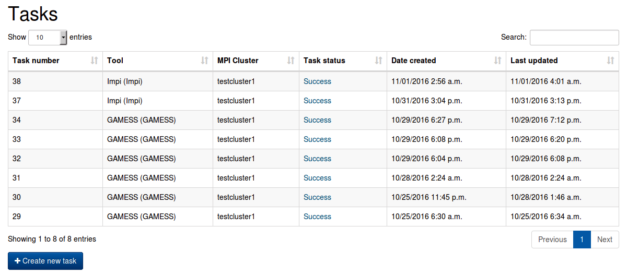
\includegraphics[scale=0.40]{./images/tasks_list_view_2.png}			
			\captionof{figure}{Task table view}			
		\end{center}	
		\item The user can view results of tasks. JSmol renders the compatible output files\cite{IJCH:IJCH201300024}. \newline
		\begin{center}			
			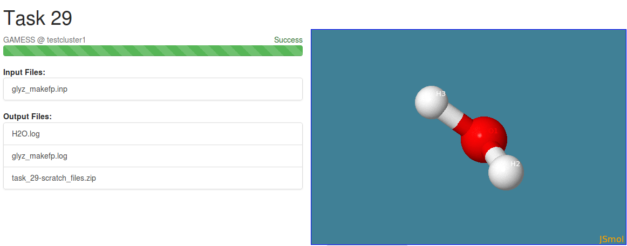
\includegraphics[scale=0.35]{./images/jsmol_detail_view_2.png}			
			\captionof{figure}{Task detail view}			
		\end{center}	

		    
		
	\end{itemize}
	
	\subsection{User Acceptance}
	\begin{center}			
			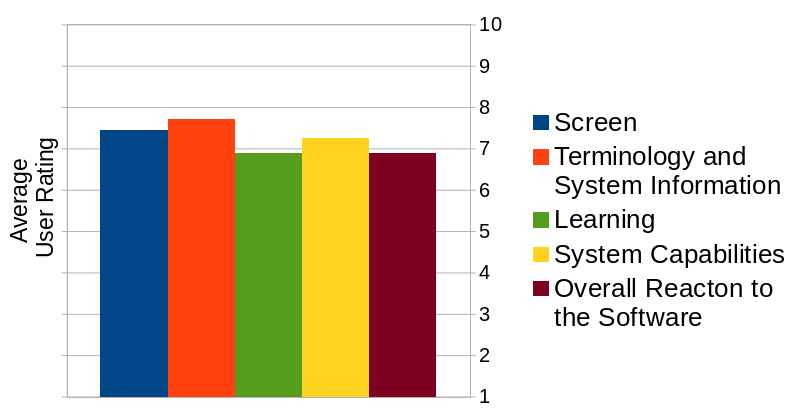
\includegraphics[scale=0.32]{./images/uat_graph.png}			
			\captionof{figure}{Results of QUIS for SkyLab}			
	\end{center}
	The system has been evaluated by 56 respondents by answering a survey based on Questionnaire for User Interface Satisfaction (QUIS) \cite{chin1988development}. Respondents are students who are unfamiliar with both HPC tools and the concept of MPI systems.  Respondents are asked to test features of SkyLab by following a set of instructions and using input files provided. On the average, the users rated their overall experience with SkyLab to 6.9/10. The users listed the simplicity of the user interface to be the most positive aspect of the system while the slow speed of task processing is said to be the most negative. Majority of the tools supported by SkyLab have inherently long processing time which is not known to the respondents. The system does not focus on optimizing the said tools to achieve better performance but rather it focuses on simplifying the user's task submission process. 

	
\section{Conclusion and Future Work}
The system created allows users to manage MPI clusters and submit tasks without the need for technical expertise in scripting. This makes the advantages of HPC available to non-technical users. This is achieved by parsing form inputs to generate commands for task execution. Task files can be download from the server and output files are displayed with the help of JSmol\cite{IJCH:IJCH201300024}. The system is also configured to install tool sets found in the modules folder making it possible to accommodate additional tools. Based on the user acceptance test conducted, the users found the system to be acceptable in terms of the criteria provided, in general. 

The system achieved its main objectives but its features can still be improved and additional features can be introduced. Improved input parameter checking and error handling will make the system more robust. There are still use cases of tools that are yet to be supported. Input file generation can make the process more interactive and more customizable.  Workflow design support will enable users to run complex tasks. Support for custom MPI programs will make it easier for developers to utilize the system as a test environment. Task scheduling and resource management algorithms can be used to efficiently handle resource-intensive or time consuming tasks. For example, a cluster can borrow resources from idle clusters. These recommendations will provide the users a better experience in using the system for academic and research purposes. 

% APPENDICES
%\appendices

%\section{Proof of the First Zonklar Equation}
%Appendix one text goes here...

%\section{}
%Appendix two (without title) text goes here...

% ACKNOWLEDGMENT
%\section*{Acknowledgment}
%Many thanks to...
% BIBLIOGRAPHY
\bibliographystyle{./IEEE/IEEEtran}
\bibliography{./carpio-cs190-ieee}
% \nocite{*}

% BIOGRAPHY
%\begin{biography}[{
\includegraphics{./yourPicture.eps}}]{Student M. Name}
%Biography text here...
%\end{biography}


\end{document}

